\subsection{Architectural Components}
In the following sections, we will discuss each one of the three components separately, starting from the lowest-level one, the Implementation system, all the way to the highest-level one, namely the API. We depict the most important classes of each one of the components in figures \ref{fig:all-classes} and \ref{fig:api-all-classes}.
\subsubsection{The Implementation system}
The Implementation system is depicted as \cb{impl} in the source code. This is the lowest-level architectural component because it is where all the functionalities that OptaPlanner provides are defined. As a reminder from previous introductory sections, the goal of OptaPlanner is to solve a problem with constraints. Therefore, the essence of such a system is to generate solutions. A solution is rendered by an entity that is called a \cb{solver}. A solver can provide several \textit{solutions} for one problem. Each solution is based on an optimization algorithm. Every running instance of an algorithm is processed via a \textit{phase}. 
Therefore, the main sub-components of this system are the {\scriptsize SOLVER} and the {\scriptsize PHASE}; the other sub-components are highly dependent on these two. Note in figure \ref{fig:impl_sys_dep} how all the arrows point towards them. \\\\
The {\scriptsize SOLVER} sub-component arranges the implementation details for the \textit{solver} entities. It uses the factory pattern\footnote{design pattern in software programming where an entity called a factory is used to instantiate classes without having to specify the exact type of the object that will be created} to instantiate solver entities automatically. However, the key component of the system is the \verb!AbstractSolver! class. This abstract class is used to implement all possible \textit{solvers} that OptaPlanner can put to use, such as a solver that applies the Partition Search algorithm, or any of the other ones (\S\ref{par:algos}). It is also used to implement the default solver (\verb!DefaultSolver.java!), the solver that does not make use of any optimization algorithms.\\\\
As we have mentioned previously, the {\scriptsize PHASE} is a crucial entity of the system because it allows for different solvers to run on the same problem, and thus, producing different possible solutions. The interface \verb!Phase.java! allows for the implementation of all different types of phases. The only parameter that it requires is the \verb!Solution_! class (\S\ref{para:solver}). Every optimization algorithm `has’ its own phase, which implements \verb!Phase.java!.
Other sub-components of the system include the ones that we have also mentioned in \S\ref{sec:arch_entities}. 
\begin{figure}
    \centering
    \subfloat{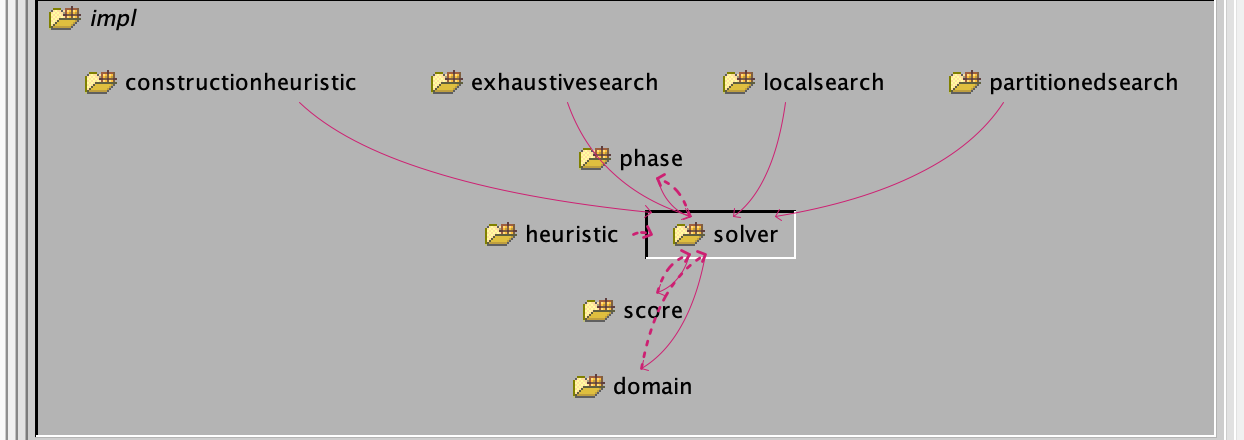
\includegraphics[width=0.6\textwidth]{figures/step2/impl:solver.png}}
    \hfill
    \centering
    \subfloat{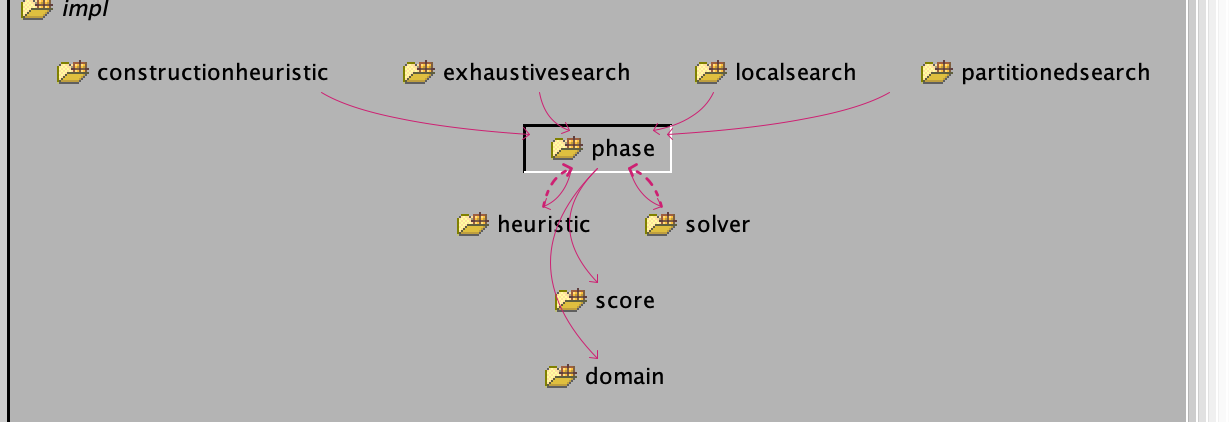
\includegraphics[width=0.6\textwidth]{figures/step2/impl:phase.png}}
    \caption{An overview of the dependency of all the components of the Implementation system on its main components, respectively: \textit{Solver} and \textit{Phase}.}
    \label{fig:impl_sys_dep}
\end{figure}
%%%%%%%%%%%%%%%%%
\subsection{The Configuration system}
\label{subsec:config_sys}
The Configuration system is depicted as \cb{config} in the source code. The main task of this system is to read the configuration details from the \verb!xml! files and convert them into useful input for the OptaPlanner software. Every input that is retrieved from the \verb!xml! files is converted into classes and objects by instantiating the classes that are implemented in the Implementation system. Therefore, the Configuration system can be also described as middleware software because it provides the overall system with the following functions:
\begin{enumerate}[label=(\roman*)]
    \item read the relevant input from \verb!xml! files 
    \item instantiate the classes of the Implementation system according to the retrieved information
    \item provide the API with configuration files that are needed by the user, in order to implement the appropriate classes for his own problem
\end{enumerate}
The main sub-component of config is the {\scriptsize SOLVER}. The {\scriptsize SOLVER} has a class called \verb!SolverConfig.java!. This class is responsible for making sure that the Solver adapts to the problem that is inputted because it is the class where all the configuration details from the \verb!xml! files are arranged. The solutions that OptaPlanner provides for the user depend on these details. An example of a \textit{Solver} configuration \verb!xml! file (that \verb!SolverConfig! class will use) can be noted in figure \ref{fig:ex_config}. We note the three main parts of the file, namely:
\begin{enumerate}[label=(\roman*)]
    \item where the model is defined: that is, the type of problem that needs to be solved. In this case, it is the NQueens problems.
    \item the score function: how should the solutions generated by OptaPlanner be assigned a fitness score?
    \item  the optimization algorithms (\S\ref{par:algos}): which algorithms should be used when generating the solutions.
\end{enumerate}
Configuration files can be updated manually if the user would like to switch between optimization algorithms. The Configuration system is crucial to OptaPlanner because, given a {\scriptsize SOLVER} and a {\scriptsize SOLUTION} (which is defined by the user), a problem can be solved by calling: \verb!NQueens bestSolution = solver.solve(problem);!\\\\
Other sub-components of the Configuration system are the:
\textit{Domain, Score, Phase, Construction Heuristics} and \textit{Algorithms}.
Essentially, the tasks of each one of these components tasks are in accordance with the ones we have introduced in section \ref{sec:arch_entities}. In this system, however, their focus lies on extracting the necessary information from the \verb!xml! files and rendering the classes and files that will be used by the API.
\begin{figure}
    \centering
    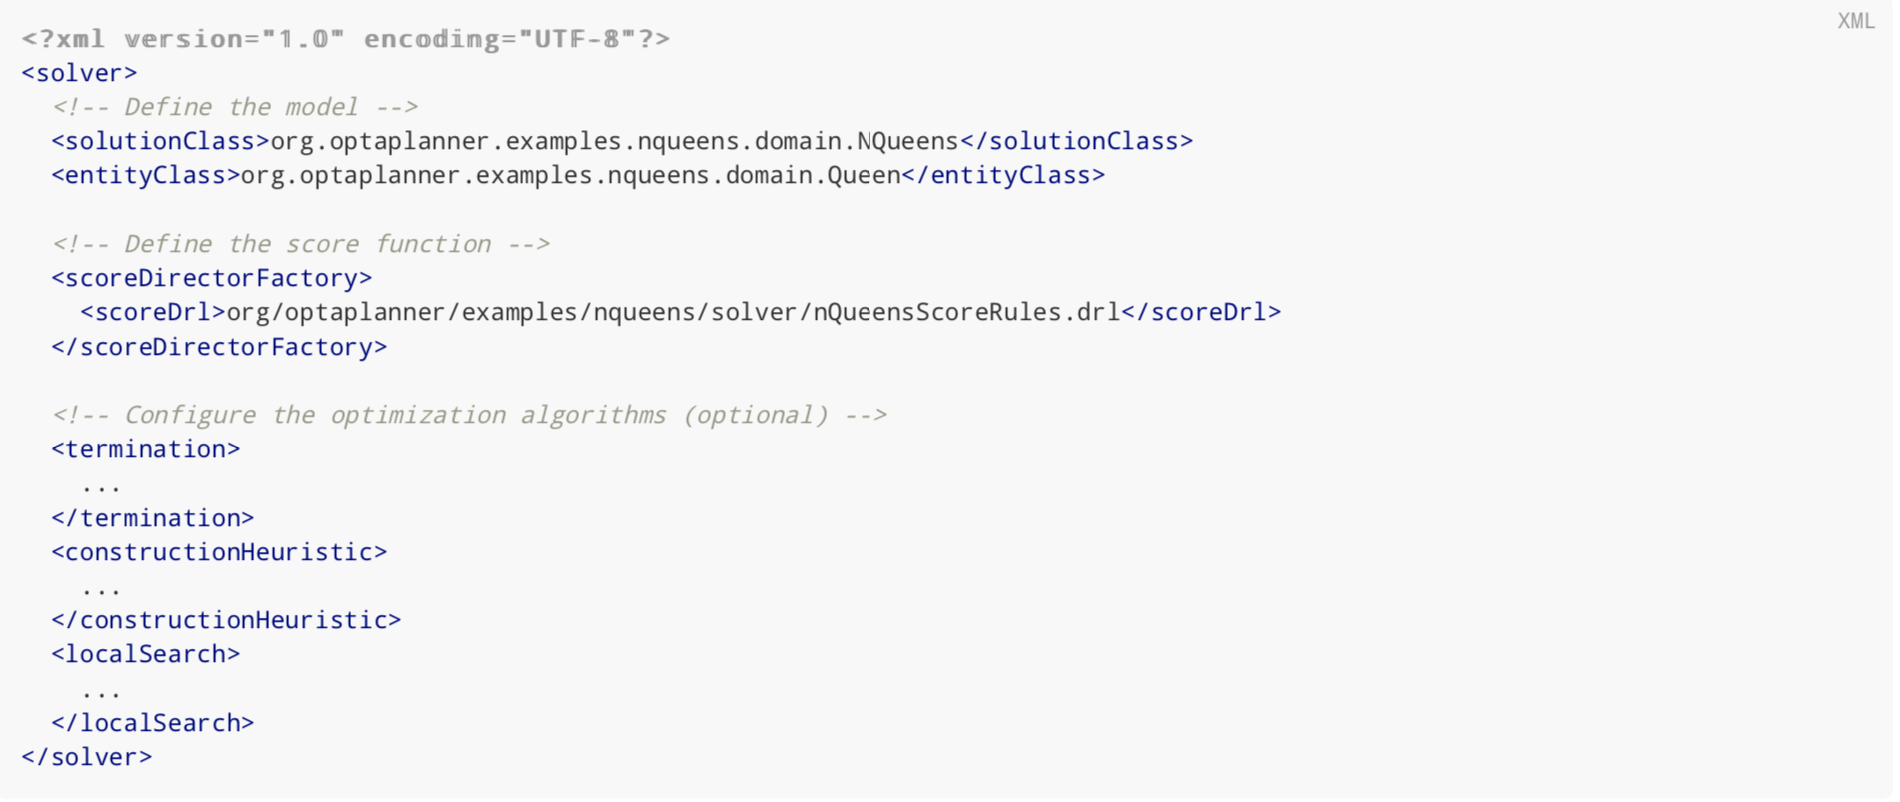
\includegraphics[width=0.8\textwidth]{figures/step2/config_file.png}
    \caption{An example of what an \textit{xml} configuration file for the NQueens problem would look like. This file represents the \textit{solver}, which will be responsible for generating solutions for the problem inputs. Note how the user can also define the optimization algorithms which he would like the solver to consider.}
    \label{fig:ex_config}
\end{figure}
\subsection{The API}
From our understanding of the source code, this architectural component is the most high-level out of the three. We believe this is the case because, if we look at the core from the viewpoint of a developer who has not worked with OptaPlanner before and wishes to use it to solve a problem that he has defined himself in \verb!Java!, then the API is, theoretically, the only component he needs to understand. All the lower-level entities (algorithms, interfaces, classes) and components of the system are `hidden’ by the API and its classes and interfaces are rather self-explanatory. More specifically, it seems that the goal of the API is to serve as an interface for implementing all the functionalities that OptaPlanner needs in order to solve a problem. These functionalities are also interfaces or classes, which can then be used by developers who would like to define their own problems. Therefore, if the Configuration system is able to parse useful information and render interfaces specific to one problem (such as NQueens), then the API is responsible for creating interfaces that will be directly used by the developers. \\\\
The key concept of this system is the \textit{Factory Pattern}, and how it is used to initiate new \textit{solvers}. There is a class called \verb!SolverFactory! which is used to initialize multiple \textit{solvers} automatically for the user. A method from the Configuration system is called, namely \verb!createFromXmlResource! of \verb!SolverConfig!. This is because the factory needs to create \textit{solver} classes that are based on the \verb!xml! details asserted by the user. The solver class of the API system is responsible for solving a planning problem and returning the best solution found, as explained in paragraph \ref{para:solver}. The \verb!solve! method (of the solver) is called by the OptaPlanner system to start the process of finding the best solution, as we also briefly mentioned in \ref{subsec:config_sys}. \\\\
In order for the system to keep track of each solution, the \verb!SolverJob! class of the API is used, where the system can have information such as whether the solution is still running or has terminated. If the user wants to have \textit{multiple solutions} of a problem being run at the same time, then he can use \verb!SolverManager! - also part of the API. This class establishes the \textit{solver factory} as we described and have each solver run a solution algorithm, always based on the \verb!xml! configuration files (which is why the \verb!SolverConfig! method is also called in here).\\\\
These are the main classes (or sub-components) of the API system. They are interfaces that the user needs to implement so that they can be applied to the \textit{domain} of his problem. For example, in our example model, we would have a \textit{Solver Factory} created specifically for NQueens, an \textit{NQueen class} that is based on the \verb!Solution_! interface where we could depict the description of the problem and its solution, and an \textit{NQueensSolver class} that implements the \verb!Solver! interface.
\subsection{Third-party components}
Essentially, the OptaPlanner system does not interact with external APIs or components. The only thing external to the \verb!core! of the system are the \verb!xml! files, since they are dynamic files that are not defined in the source code. Instead, they are read and processed runtime in the Configuration system when the software is trying to solve a problem. By using generic classes (like \verb!Solution_!), the system can use annotations to mark the methods and classes that are concerned with the processing of the information from the \verb!xml! files. More specifially, for the time being, OptaPlanner is using the \verb!XStream! annotation services. Other than this, all the functionalities that the software uses to provide results for the user are developed by the development team of OptaPlanner.
\begin{figure}
    \subfloat[\label{subfig:config-classes}]{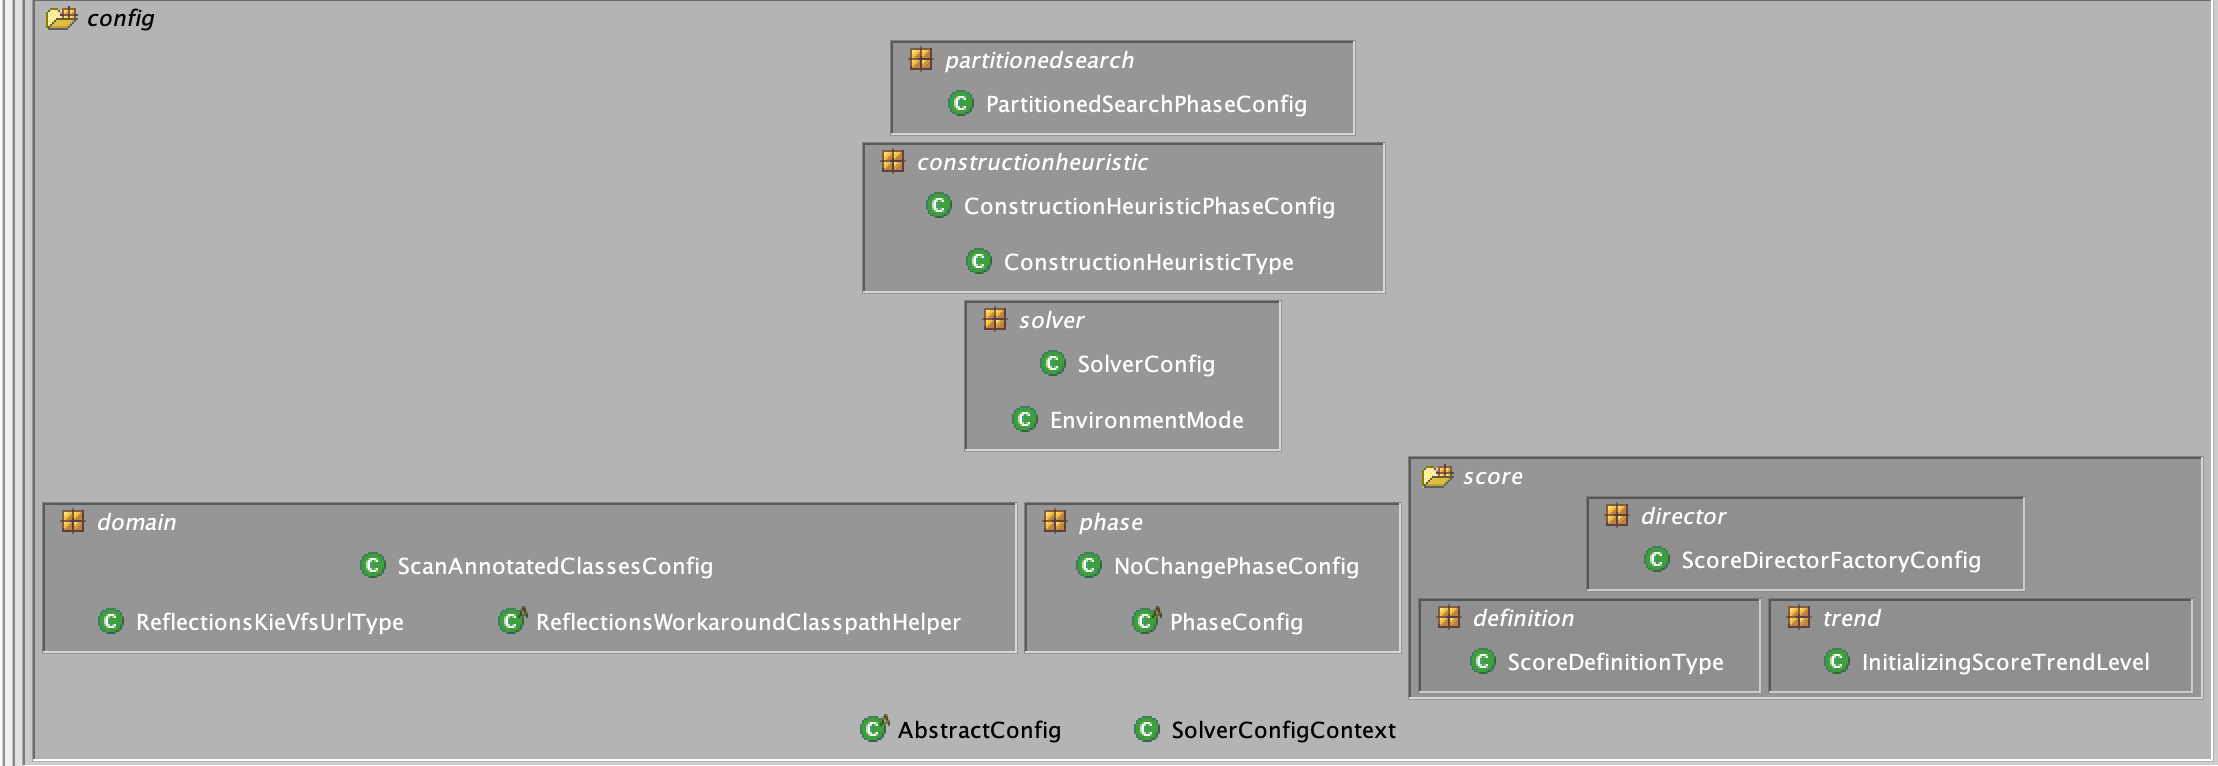
\includegraphics[width=\textwidth]{figures/step2/config-all-classes.png}}
    \hfill
    \subfloat[\label{subfig:impl-classes}]{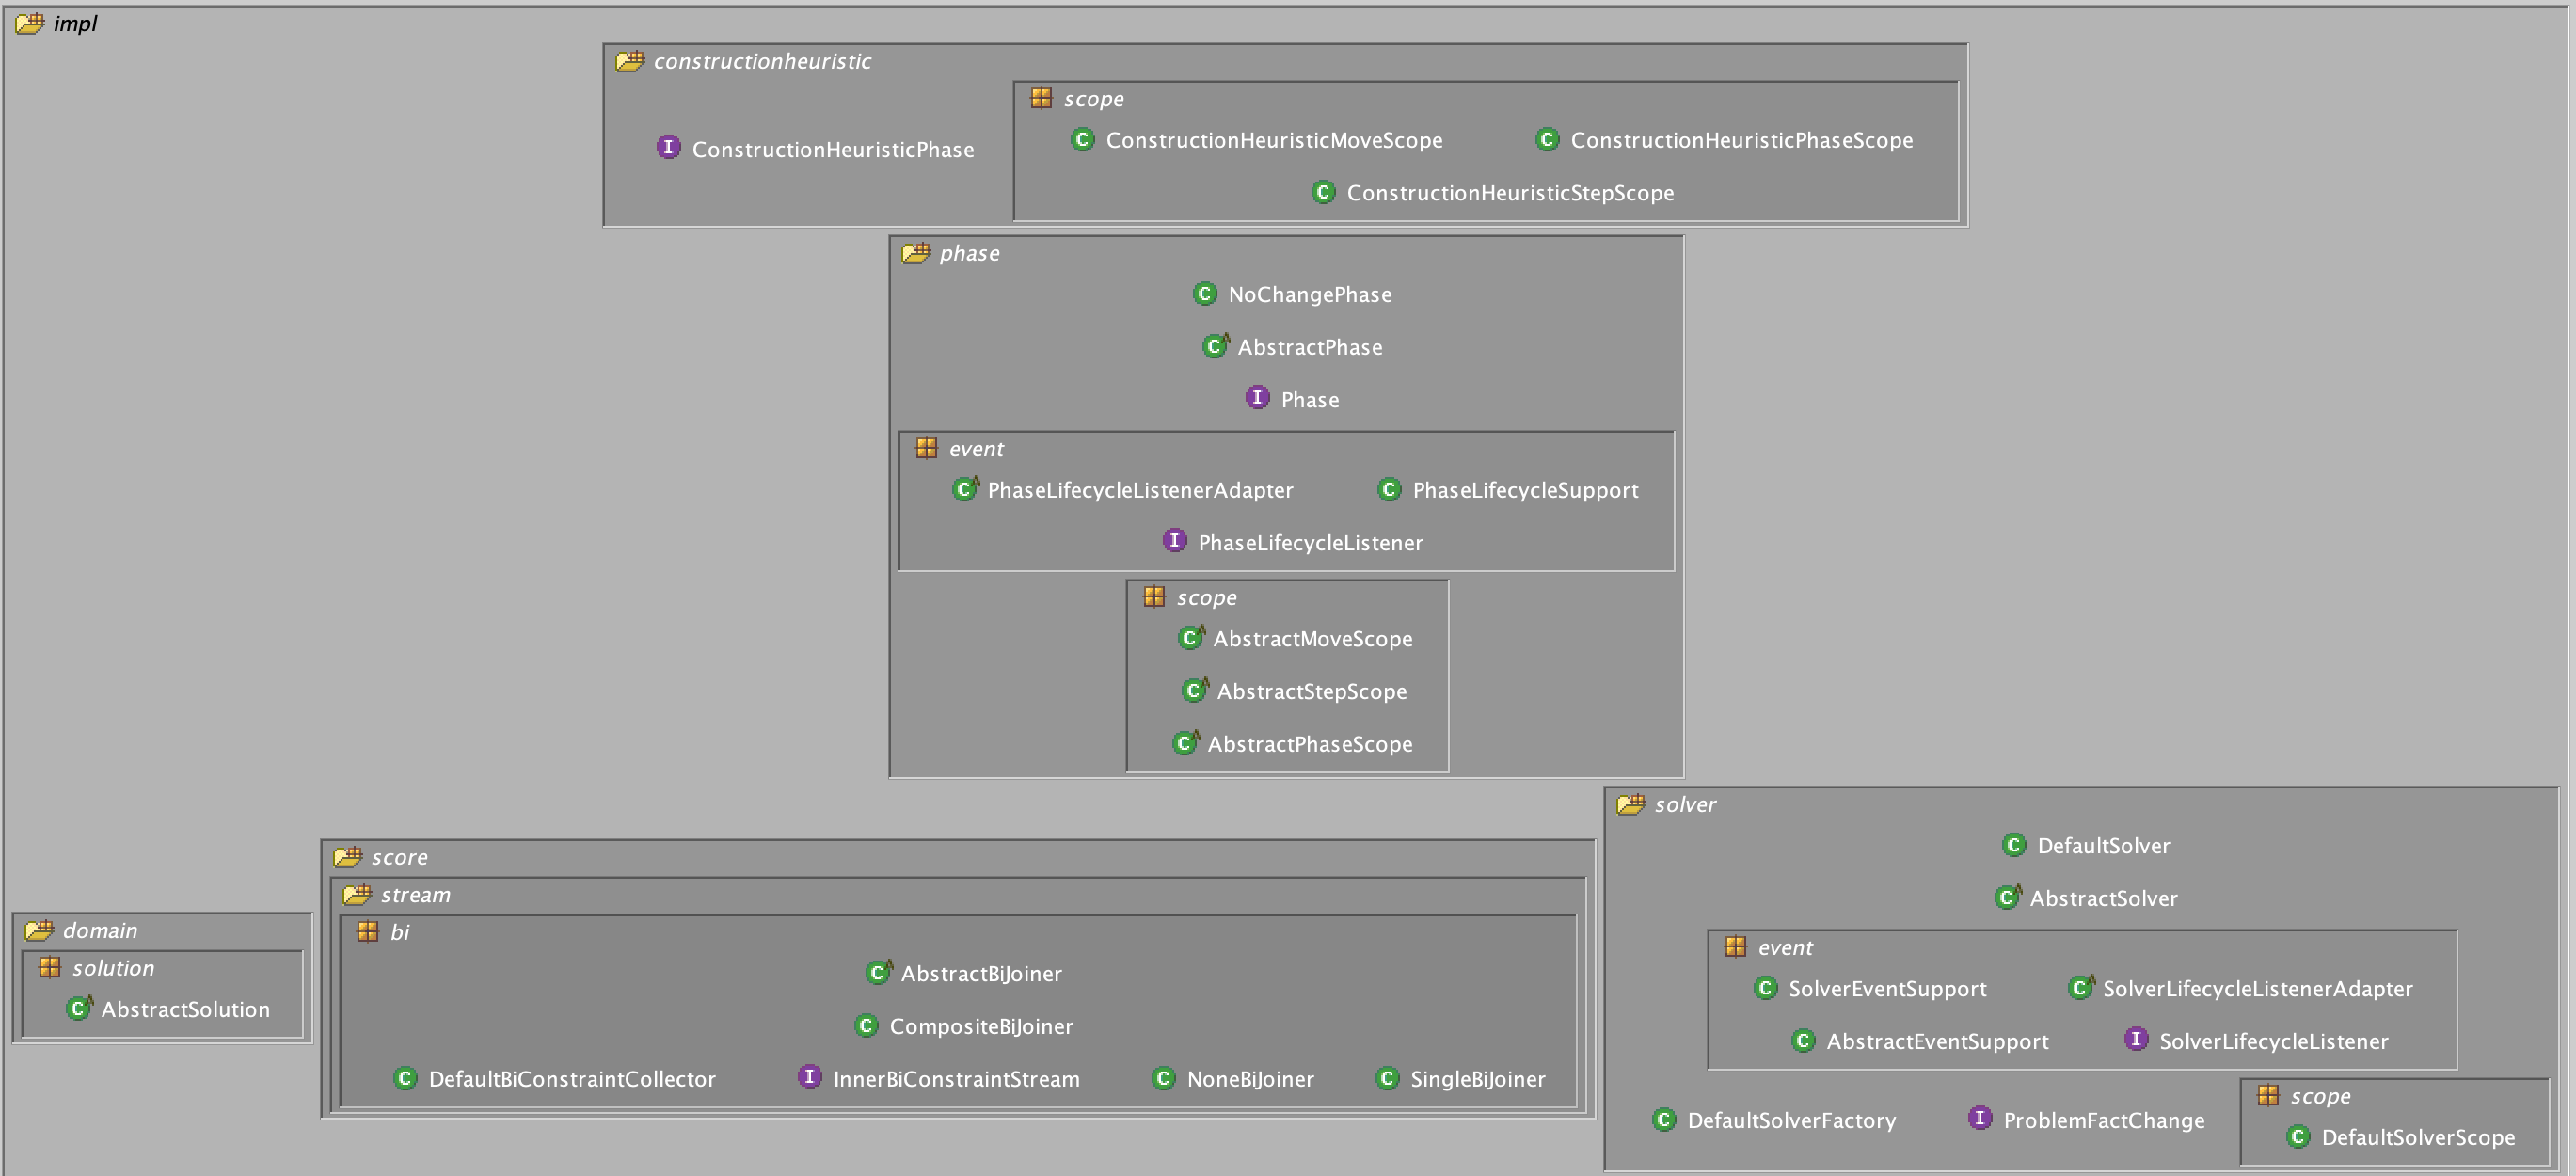
\includegraphics[width=\textwidth]{figures/step2/impl-all-classes.png}}
    \caption{The first diagram depicts all the important classes of the Configuration system, including their packages. The second diagram depicts all the classes of the Implementation system.}
    \label{fig:all-classes}
\end{figure}
\begin{figure}
    \centering
    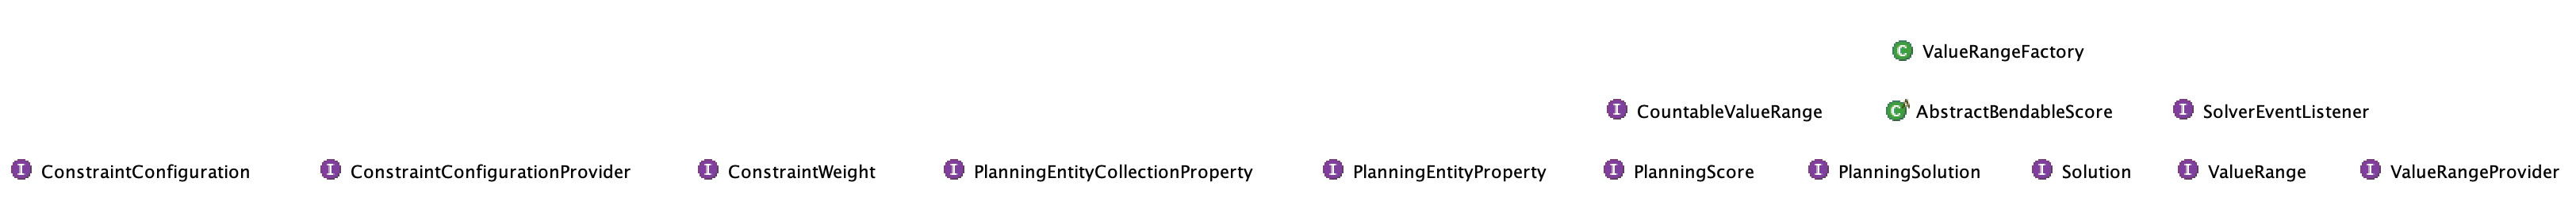
\includegraphics[width=\textwidth]{figures/step2/api-all-classes1.png}
    \caption{A diagram of the most relevant classes of the API, depicted without their packages.}
    \label{fig:api-all-classes}
\end{figure}